\section{Introduction} \label{introduction} 

We show how the task of finding equivalent
mathematical expressions can be automated. Our focus is on finding equivalent
mathematical formulas (i.e.~which give an identical numerical result
to the original expression) for marginalization over huge sets. 
Problems of marginalization are prevalent in machine learning, and 
exact marginalizations can be a replacement for sampling methods.



We propose a deterministic, grammar-based framework which discovers
relations between multi-variable polynomial expressions. First, we
construct an attribute grammar -- a context-free grammar extended to
contain set of attributes, introduced by Donald Knuth
\cite{knuth1968semantics}. To define the search space we use a set of
context-free grammar rules representing admissible operations. 



\begin{minipage}{\linewidth}
\begin{framed}
\begin{flushleft}
We are given matrices $A \in \mathbb{R}^{n \times m}$, $B \in \mathbb{R}^{m \times k}$. We wish
 to compute \texttt{sum(sum(A*B))}, i.e.~: 
\vspace{1.5mm} \\ 
$\sum_{n,k} AB = \sum_{i = 1}^n \sum_{j = 1}^m \sum_{l = 1}^k A_{i, j} B_{j, l} $
\vspace{1.5mm} \\ 
which naively takes $O(nmk)$ time. Our framework is able to discover
an efficient version of the formula, that computes the same result in $O(n(k+m))$
time:
 \vspace{1mm} \\
%\begin{verbatim}
\texttt{	sum(sum(A .* repmat(sum(B, 2), [1, n])'))}
 \vspace{1mm} \\ 
Our framework has four distinct stages:
 \begin{enumerate}
\item The {\em grammar tree} is built (see Algorithm 1). This contains
  an exhaustive set of all valid compositions of expressions from the
  grammar. While slow, this only needs to be performed once for a
  given grammar, irrespective of the number of target expressions we
  wish to compute. The figure below shows two branches of the grammar
  tree.
\item Framework looks for linear combination of tree leafs 
  to match target expression. This may require solving a linear system.
  It chooses leafs with smallest computational complexity 
  (see Section \ref{sec:linear}). The two leaves \texttt{L$_1$} and
  \texttt{L$_2$} shown in the tree produce the same result as the target
  expression. 
\end{enumerate}

Empirical tests indicate that our expression is indeed faster to
compute than the naive one (see Figure \ref{ab}).

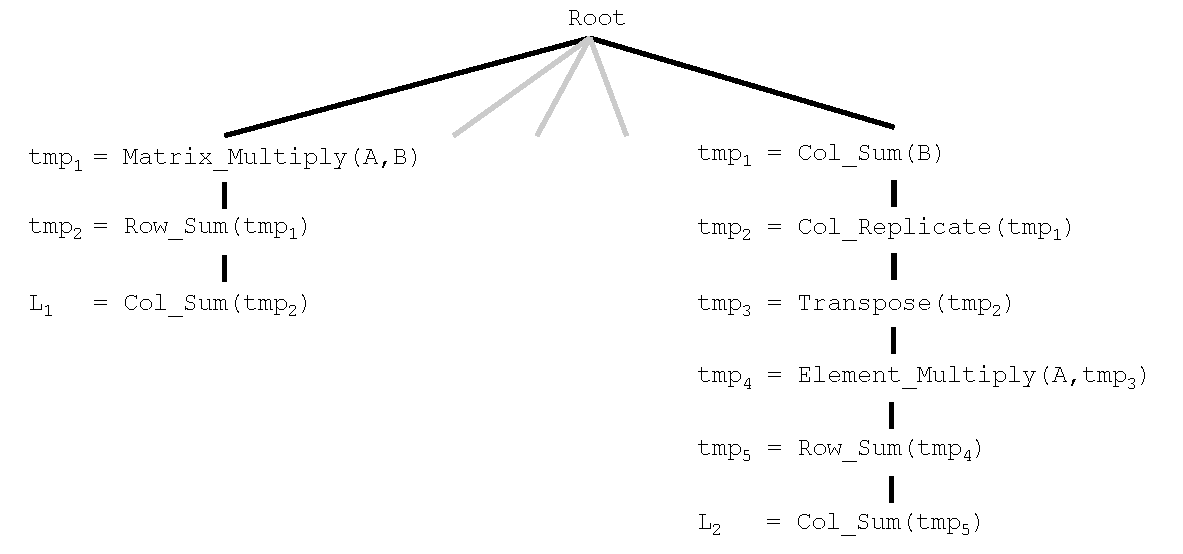
\includegraphics[scale=0.4]{img/toy_tree.pdf}
\end{flushleft}
\end{framed}
%\caption{Presents how framework works to compute fast expression sum(sum(A*B)).}
\label{fig:example_ab}
\end{minipage}


\noindent
By representing the cost of every operation as a synthesized attribute
(i.e. computed bottom-up from child node attributes) we can search for
formula with low time complexity. Through a linear combination of
grammar elements, we can find a solution to the desired
expressions. 



Figure \ref{fig:example_ab} shows our framework applied to a simple matrix expression:
\texttt{sum(sum(A*B))}, where \texttt{A} and \texttt{B} are matrices. Naively, this takes $O(n^3)$ to compute due to
the matrix multiply operation. The example outlines how our framework
can find an alternate way of computing {\em exactly} the same result,
but in $O(n^2)$ time. We start with this simple (non-machine learning example) to
explain how system works.

We demonstrate the flexibility of our technique by applying it to 
various problems in machine learning: 
\begin{enumerate}
\vspace{-2mm}
\item Exact summation for RBM partition function like expression. We can produce an exact 6th order 
  Taylor of RBM partition function approximation which is
  computable in closed-form, and takes polynomial time.
  Naive evaluation of the Taylor-series
  approximation would require summing over the $2^n$ possible states.   
\item Closed-form computation of Dropout for rational activation functions. 
  Dropout \cite{hinton2012improving}
  involves the  stochastic deletion of outputs within a dense neural
  network layer at training time. For $n$ output units, the $2^n$
  possible deletion patterns are sampled independently for each
  training sample. We use our framework to derive a closed-form
  expression that integrates out over all $2^n$ states (Section \ref{sec:dropout}).
\item Data augmentation is for object recognition purposes it consists
  translations, rotations, contrast alternation and few others. 
  We how to construct update rule to weights which
  integrates over all contrast alternations (Section \ref{sec:augm}).
\end{enumerate}
\vspace{-2mm}

The main contribution of the paper is the introduction of a general
framework for discovering efficient closed-form expressions. This are
of the main use for marginalization problems (or sum over large number of
expressions). Its
flexibility means can be used on a wide range of problems encountered
in math and AI, beyond those outlined above. We dedicate follow up 
papers to address properly each of aforementioned applications. This
paper focuses mainly on framework description, and gives only brief description
of applications. By the time of publication, we will release Matlab and python
code to generate computations described in this paper.

